%----------------------------------------------------------------
%
%  File    :  chapter3.tex
%
%  Authors :  Michael Fuska, FH Campus Wien, Austria
% 
%  Created :  08 Feb 2016
% 
%  Changed :  
% 
%----------------------------------------------------------------


\chapter{iOS}
\label{chap:iOS}

\section{iOS Grundlagen}
\label{sec:iOSGrundlage}

Das mobile Apple Betriebsystem iOS basiert auf dem Desktop Betriebssystem des Mac OS X. Darwin ist ein frei erhältliches Linux basiertes Betriebssystem. Dieses Betriebssystem stellt die Grundlage für das Mac OS X dar. Der Kernel des Mac OS X ist der XNU-Kernel mit entsprechenden Adaptionen für das Mac OS X und dem mobilen Betriebssystem iOS.
\begin{figure}[htbp]
        \centering
                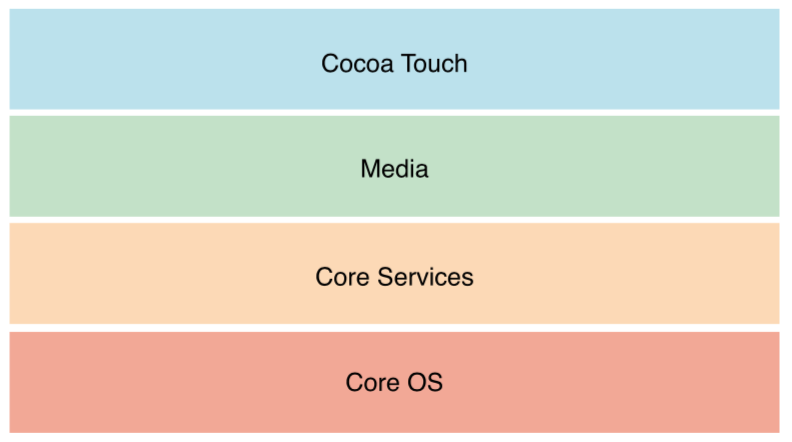
\includegraphics[height=5cm]{Bilder/Chapter3_SystemArchitektur}
        \caption{iOS Software Layer\cite{Apple[6]} }
        	\label{fig:iOS Software Layer}
\end{figure}
Die abgebildeten Schichten zeigen das abstrahiert iOS Betriebssystem. Der grösste Unterschied zwischen Mac OS X und iOS liegt im Layer Cocoa Touch.


\begin{description}
 	\item[iOS Software Layer]~\par
	\begin{itemize}
	
		%---------------------------------- Core OS ------------------------------------
      		\item \textbf{Core OS Layer} \\
		Der Core OS Layer beinhaltet alle low-level Features und auf diesen bauen alle anderen Frameworks auf. iOS Applikationsentwickler kommen mit diesem Layer nur dann in Berührung, wenn sie sich mit der Sicherheit und mit Hardware-Kommunikation beschäftigen. Dieser Layer stellt folgende
		\begin{description}
			\item[\glqq Frameworks\grqq{}]~\par
			\begin{itemize}
				\item Accelerate Framework
				\item Core Bluetooth Framework
				\item External Accessory Framework
				\item Generic Security Service Framework
				\item Lost Authentication Framework
				\item Network Extension Framework
				\item Security Framework
				\item System
				\item 64-Bit Support
			\end{itemize}
		\end{description}
		zu Verfügung. 
		
		%---------------------------------- Core Service ------------------------------------
         	\item \textbf{Core Service Layer} \\
		Der \glqq Core Service Layer\grqq{} beinhaltet die fundamentalen System Service. Dieser Layer wird unterteilt in High-Level Feature und Core Services Frameworks.
		\begin{description}
			\item[\glqq High-Level Feature\grqq{}]~\par
			\begin{itemize}
				\item Peer-to-Peer Services
				\item iCloud Storage
				\item Block Objects
				\item Data Protection
				\item File-Sharing Support
				\item Grand Central Dispatch
				\item In-App Purchase
				\item SQLite
				\item XML Support 
			\end{itemize}
			\item[\glqq Core Services Framework\grqq{}]~\par
			\begin{multicols}{2}
			\begin{itemize}
				\item Accounts Frameworks
				\item Address Book Framework
				\item Ad Support Framework
				\item CFNetwork Framework
				\item CloudKit Framework
				\item Core Data Framework
				\item Core Foundation Framework
				\item Core Location Framework
				\item Core Media Framework
				\item Core Motion Framework
				\item Core Telephony Framework
				\item EvenKit Framework
				\item Foundation Framework
				\item HealthKit Framework
				\item HomeKit Framework
				\item JavaScript Framework
				\item Mobile Core Services Framework
				\item Multipeer Connectivity Framework
				\item NewStandKit Framework
				\item PassKit Framework
				\item Quick Look Framework
				\item Safari Services Framework
				\item Social Framework
				\item StoreKit Framework
				\item System Configuration Framework
				\item WebKit Framework
			\end{itemize}
			\end{multicols}
		\end{description}

		%---------------------------------- Media Layer ------------------------------------
         	\item \textbf{Media Layer} \\
		In diesem Layer sind alle Technologien zur Darstellung von Grafik, Video und Sound enthalten. Dieser Layer ist verantwortlich für das Design und den Sound der iOS Applikationen.  
		Dieser Layer stellt folgende
		\begin{description}
			\item[\glqq Technologien\grqq{}]~\par
			\begin{itemize}
				\item Graphics Technologies
				\item Audio Technologies
				\item Video Technologies
				\item AirPlay
			\end{itemize}
		\end{description}
		zur Verfügung.
		
		\begin{description}
		\item[Folgende Frameworks beinhaltet dieser Layer]~\par
		\begin{multicols}{2}
		\begin{itemize}
			\item Assets Library Framework
			\item AV Foundation Framework
			\item AVKit Framework
			\item CoreAudioKit Framework
			\item Core Graphics Framework
			\item Core Image Framework
			\item Core Text Framework
			\item Core Video Framework
			\item Game Controller Framework
			\item GLKit Framework
			\item Image I/O Framework
			\item Media Accessibility Framework
			\item Media Player Framework
			\item Metal Framework
			\item OpenGL ES Framework
			\item Photos Framework
			\item Photos UI Framework
			\item Quartz Core Framework
			\item SceneKit Framework
			\item SpriteKit Framework
         	\end{itemize}
		\end{multicols}
		\end{description}
		%---------------------------------- Cocoa Touch Layer ------------------------------------
		\item \textbf{Cocoa Touch Layer}\\
		Enthält die wichtigsten Frameworks um iOS Applikationen zu entwickeln. Dieser Layer stellt die Basis Applikation Infrastruktur und
		\begin{description}
			\item[die \glqq Key Technologien\grqq{}]~\par
			\begin{itemize}
				\item Multitasking
				\item touch-based input
				\item push notification
				\item \glqq high-level\grqq{} System Service
			\end{itemize}
		\end{description}
		zu Verfügung. 
		
		\begin{description}
		\item[Folgende Features sind in diesem Layer enthalten]~\par
		\begin{multicols}{2}
		\begin{itemize}
			\item App Extentision
			\item Handoff
			\item Document Picker
			\item AirDrop
			\item TextKit
			\item UIKit Dynamics
			\item Multitasking
			\item Auto Layout
			\item Storyboards
			\item UI State Preservation
			\item Apple Push Notification Service
			\item Local Notifications
			\item Gesture Recognizers
			\item Standard System View Controllers
         	\end{itemize}
		\end{multicols}
		\end{description}
		\begin{description}
		\item[Folgende Frameworks beinhaltet dieser Layer]~\par
		\begin{multicols}{2}
		\begin{itemize}
			\item Address Book UI Framework
			\item EventKit UI Framework
			\item GameKit Framework
			\item iAd Framework
			\item MapKit Framework
			\item Message UI Framework
			\item Notification Center Framework
			\item PushKit Framework
			\item Twitter Framework
			\item UIKit Framework
         	\end{itemize}
		\end{multicols}
		\end{description}

         \end{itemize} 
\end{description}

%----------------------------------------------------------------

\section{iOS Security Architektur}
\label{sec:iOSSecArchitektur}

Die Sicherheitsmechanismus der iOS Device unterteilt sich in zwei Ebenen. 
\begin{figure}[htb]
  \begin{minipage}{0.6\textwidth} 
  		\begin{description}
   			\item[ iOS Sicherheitsebenen]~\par
         		\begin{enumerate}	
				\item  \textbf{iOS Software}
					\begin{enumerate}
       						\item File System
         					\item OS Partition
						\item User Partition (verschlüsselt)
						\item App Sandbox
						\item Data Protection Class
      					\end{enumerate}
      				\item  \textbf{iOS Hardware und Firmware}~\par
					\begin{enumerate}
       						\item Kernel
						\begin{enumerate}
						\item Secure Enclave
						\item Secure Element
         					\end{enumerate}	
						\item Crypto Engine
						\item Device Key
						\item Group Key
						\item Apple Root Certificate
      					\end{enumerate}
			\end{enumerate}
   		\end{description}
Die iOS Sicherheit passiert auf der Kombination von Software, Hardware und Services um ein maximum an Sicherheit zu erreichen.
	% \caption{Der Text}
	% \label{Text}
	\end{minipage}
	% Auffüllen des Zwischenraums
	\hfil
	% minipage mit Grafik
	\begin{minipage}{0.4\textwidth}
		% \textwidth bezieht sich nun auf die Minipage
		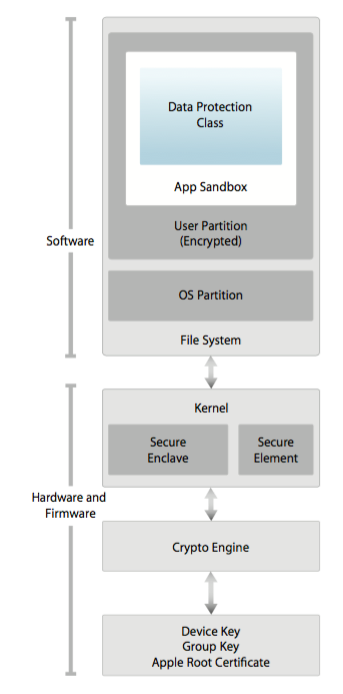
\includegraphics[width=\textwidth]{Bilder/Chapter3_SecArchitektur}
		\caption{iOS Security Architektur \cite{Apple[4]} }
        		\label{fig:iOS Security Architektur}
	\end{minipage}
	% \caption{noch eine Caption}
\end{figure}
		    	
%----------------------------------------------------------------
\section{System Security}
\label{sec:SystemSec}

\subsection{Secure boot chain}
\label{subsec:SystemBootChain}

\subsection{System Software Authiruzation}
\label{subsec:SystemSWAuth}

\subsection{Secure Enclave}
\label{subsec:SystemSecEnclave}

\subsection{Touch ID}
\label{subsec:SystemTouchID}

%----------------------------------------------------------------
\section{Encryption und Daten Sicherheit}
\label{sec:DataEnc}

%----------------------------------------------------------------
\section{Applikation Security}
\label{sec:AppSec}

%----------------------------------------------------------------
\section{Network Security}
\label{sec:NetworkSec}

%----------------------------------------------------------------
\section{Device Controls}
\label{sec:DeviceControl}

%----------------------------------------------------------------
\section{Privacy Controls}
\label{sec:}


